\chapter{Evaluation}
This chapter evaluates my implementation of the telecommunication
analyzer and its functionality in terms of a scan and an analyze
process. These operations are performed by executing the compiled
binary, \textbf{telecan}, with a set of options as listed in
\cref{fig:usage}. As of this writing, the binary currently depend on
GNU Radio, Boost C++ library and libhackrf to be available on the
system and the build process is only tested on OS X. A refractional
resampler and low pass filter is linked from GNU Radio as part of the
downsampling process. These dependencies are meant as a temporary test
environment and is planned to be dropped in turn for filter
implementations specific to this application.

\begin{figure}[H]
  \centering
  \begin{BVerbatim}
Usage:
    Base Station scan:
          telecan -s <band indicator>

    Tune to channel frequency:
          telecan -b <band indicator> -c <channel number>

Where options are:
    -s    band to scan (GSM850, GSM-R, GSM900, EGSM, DCS, PCS)
    -c    channel of nearby GSM base station
    -b    band indicator (GSM850, GSM-R, GSM900, EGSM, DCS, PCS)
\end{BVerbatim}
  \caption{A set of options supported by the \textbf{telecan} binary.}
  \label{fig:usage}
\end{figure}

With the libraries available, the scan and analyze can be
executed. The scan process is solely meant for \gls{BTS} searches
which, after completion, informs about nearby \gls{GSM} channels and
their corresponding frequencies and calculated frequency offset. Such
a scan is performed and illustrated in \cref{fig:scan} on the
\gls{GSM} 1800$\si{MHz}$ band in Nærum, Denmark and the channel number
refers to the \gls{ARFCN} identity.

Three attempts are made for each channel with a new set of samples to
improve the certainty that the result is in fact a \gls{FCCH}
channel. An uncertainty exists for some sequences of samples with an
oversampling ratio of four and this causes trouble during
synchronization. Feedback about phase offset is required which the
application currently does not provide.

\begin{figure}[H]
  \centering
  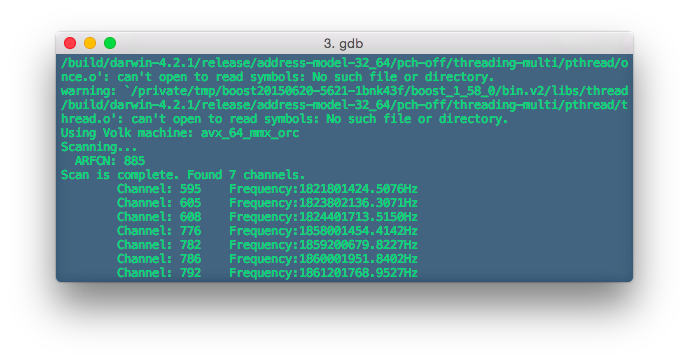
\includegraphics[width=0.75\textwidth]{figures/scan}
  \caption{A successful scan action that finds nearby channels on the
    GSM $1800\si{MHz}$ band.}
  \label{fig:scan}
\end{figure}

With a list of known nearby channels, the full synchronization process
can be initiated with the band- and channel options and the
application attempts to find the frequency correction channel again,
correct the frequency offset and search for the synchronization
channel. \cref{fig:sch_decode} illustrates a succesful
synchronization process which then continues into a failing stage for
the following estimations of normal bursts. The application attempts
to resynchronize with new samples when ten failures occur.

After the \gls{SCH} search the application attempts to decode the
following bursts in the remaining timeslots before returning to
timeslot $0$ and these are stored over a sequence of four consecutive
\gls{TDMA} frames. By examining this situation, an array of four
bursts is attempted to be decoded. \cref{fig:bad_estimation} shows the
midamble of these bursts and how they are incorrectly estimated
compared to the known training sequence at the bottom.

\begin{figure}
  \centering
  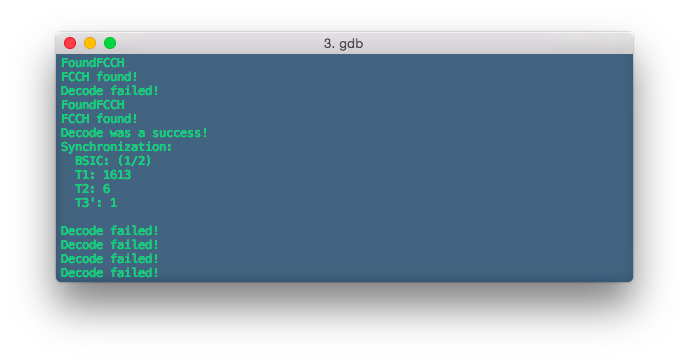
\includegraphics[width=0.75\textwidth]{figures/successful_sch_decode}
  \caption{A succesful synchronization and parsed burst information.}
  \label{fig:sch_decode}
\end{figure}

The first two bursts are completely off, which could be caused by an
incorrectly estimation of the impulse response. The exact reason is
yet to be discovered however.

\begin{figure}[H]
  \centering
  \begin{BVerbatim}
... 000000000000000000000000000000000000000000000000000000000000 ...
... 000000000000000000000000000000000000000000000000000000000000 ...
... 110111111000011110111101111100010110011010000010110001000110 ...
... 101010001001100110011000010100010111011010111100101011110010 ...
                     01000011101110100100001110
  \end{BVerbatim}
  \caption{A midamble sequence of four bursts over four frames in
    timeslot $0$ that shows a misestimation of bits. The training
    sequence at the bottom should have been visible at the same offset
    in all four sequences.}
  \label{fig:bad_estimation}
\end{figure}

With just a partly working application, as of this writing, there is much
work to be done in the future. This leads to the next chapter which
walks through a list of examples and ideas of what to work on in the
future.
